% =============================================================================
% Project : THE_PHILOSOPHY_OF_VIABILITY
% Book    : Book I — Ontology of Viability
% Book ID : VS.B01
%
% File    : 4_ASSETS/illustrations/
%           VS.B01.P01.C03.S04.SS08.P003.IL01.multiple_identity_attributions_within_one_configuration.tex
%
% Asset   : IL01 — Multiple Identity Attributions Within One Configuration
%
% Purpose :
%   To provide an intuitive illustration of how several
%   distinguishable elements may participate in one broader
%   configuration while the identity status of the elements
%   and the configuration remains a separate question.
%
% =============================================================================

\begin{figure}[htbp]
\centering

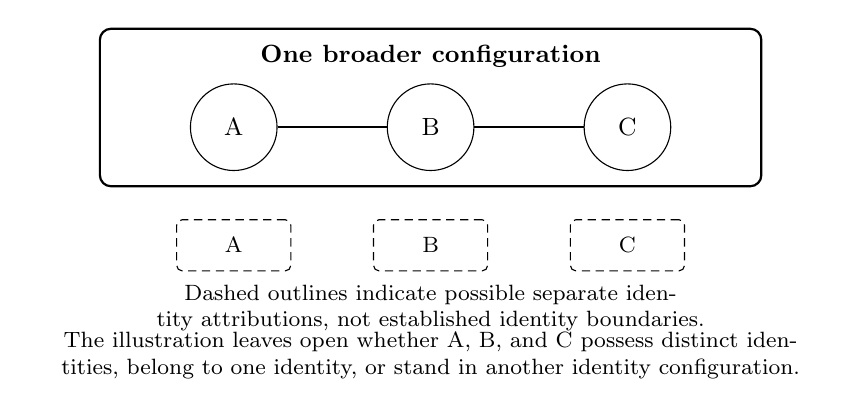
\begin{tikzpicture}[
    element/.style={
        circle,
        draw,
        minimum size=11mm,
        font=\small
    },
    possible/.style={
        draw,
        densely dashed,
        rounded corners=2pt,
        minimum width=1.45cm,
        minimum height=0.65cm,
        font=\footnotesize
    }
]

% Broader configuration
\draw[thick, rounded corners=4pt]
    (-4.2,1.0) rectangle (4.2,-1.0);

\node[font=\small\bfseries] at (0,0.65) {
    One broader configuration
};

% Elements within the configuration
\node[element] (a) at (-2.5,-0.25) {A};
\node[element] (b) at (0,-0.25) {B};
\node[element] (c) at (2.5,-0.25) {C};

\draw[thick] (a) -- (b);
\draw[thick] (b) -- (c);

% Possible identity attributions
\node[possible] at (-2.5,-1.75) {
    A
};

\node[possible] at (0,-1.75) {
    B
};

\node[possible] at (2.5,-1.75) {
    C
};

\node[
    align=center,
    text width=10cm,
    font=\footnotesize
] at (0,-2.55) {
    Dashed outlines indicate possible separate identity
    attributions, not established identity boundaries.
};

\node[
    align=center,
    text width=10cm,
    font=\footnotesize
] at (0,-3.15) {
    The illustration leaves open whether A, B, and C
    possess distinct identities, belong to one identity,
    or stand in another identity configuration.
};

\end{tikzpicture}

\caption{A unified configuration with identity attributions left open}
\label{fig:multiple-identity-attributions-within-one-configuration}

\end{figure}

% =============================================================================
% END OF ASSET IL01
% =============================================================================